\documentclass[a4paper,english]{ifimaster}

\usepackage[utf8]{inputenc}
\usepackage{babel,duomasterforside}
\usepackage{hyperref}
\usepackage{pdfsync}
\usepackage{wrapfig}
\usepackage{csquotes}
\usepackage{graphicx}
\usepackage{minted}
\usepackage{varioref}
\usepackage{parskip}
\usepackage[backend=biber]{biblatex}
\usepackage[toc,page]{appendix}

\addbibresource{citations.bib}
\graphicspath{ {./illustrations/} }

\newcommand{\todo}[1]{\textcolor{red}{[[TODO: #1]]}\PackageWarning{TODO:}{#1!}}

\title{Three Way Merge for Feature Model Evolution Planning}
\date{May 2021}
\author{Eirik Halvard Sæther}
\synctex=1

\begin{document}

\duoforside[dept={Department of Informatics},
program={Informatics: Programming and Systems Architecture},
long]
\frontmatter{}

\chapter*{Acknowledgements}

Thanks to Ida

Thanks to Ingrid and Crystal

Thanks to Germans, everyone on the LTEP project for input etc.

Thanks to ifi, all the people i have met

Thanks to friends and family

\newpage
\thispagestyle{empty}
\mbox{}
\chapter*{Abstract}

\todo{write abstract}

Feature Model Evolution Plans is intended to help ease the development of software product lines (SPLs). Feature Models allow software engineers to explicitly encode the similarities and differences of an SPL. However, due to the changing nature of an SPL, Evolution Plans allows for representing the \textit{evolution} of a feature model, not just the feature model as a single point in time.

Evolution planning of an SPL is often a dynamic, changing process, due to changing demands of the focus of development. The evolution planning is often not just done by a single engineer, but multiple engineers, working separately and independent of each other. Due to these factors, the need to unify and synchronize the changes the evolution plan emerges.

In this thesis, we develop a merge tool for Feature Model Evolution Plans. The core of the tool is a three-way merge algorithm. Given two different versions of an evolution plan, together with the common evolution plan they were derived from, the merge algorithm will attempt to merge all the different changes from both versions. If the merges are unifiable, the algorithm will succeed and yield the merged result containing the changes from both versions. However, if the changes are conflicting in any way, breaking the structure or semantics of evolution plans, the algorithm will stop, telling the user the reason of failure.

\tableofcontents{}
\listoffigures{}
\listoftables{}

\chapter*{Preface}

\todo{write better and more}
something about the LTEP project

something about summer project?

\mainmatter{}

\chapter{Introduction}%
\label{cha:introduction}

A \textit{Software Product Line (SPL)} is a collection of closely-related software products. The different software products in the SPL have several things in common, as well aspects that separate them. As an software development paradigm, SPLs allows the developers to leverage the softwares commonalities and variabilities in order to improve a variety of factors.

This variability and commonalities can be captured by \textit{feature models (FM)}, which uses \textit{features} to capture the different aspects of an SPL. Each feature in the feature model corresponds to a certain increment in program functionality. The particular \textit{variant} of the software product line is defined by a unique combination of features \cite{cite:don_batory_fm_grammar_prop}. The feature model organizes the features in a tree structure to capture the variability of the SPL.

Since SPLs undergo continuous evolution, planning for the long-term evolution of a software product line is often crucial. The evolution of the SPL is mostly handled as an informal procedure relying on the intuition and experience of individual engineers. Without formal tools, long-term goals might not be addressed properly, increasing the risk of significantly increased development costs.

We address the lack of tools for long-term evolution planning with \textit{feature model evolution plans}, or just \textit{evolution plans}, which not only models the current feature model, but all intended future feature models. This allows engineers as well as non-technical stakeholders to have a concrete tool for planning the long-term development of the software product line. The evolution plan makes it possible to plan when certain features are introduced or removed, or simply changing the way the features are related to each other. 

Planning the evolution of the software product line often involves multiple engineers changing and evolving the plan. Therefore, creating tools for evolution planning requires synchronization techniques for allowing collaborators to work independently. Naively integrating each persons changes to the evolution plan may yield inconsistencies and conflicts, so we investigate different merging strategies to ensure a sound, well-formed evolution plan is produced after the merge.

\todo{scope: her modellerer jeg bare planlegging.}
\todo{hvordan min oppgave skal leses.}

\section{Motivation}%
\label{sec:motivation}

Evolution plans are designed to help engineers cope with the long-term evolution of software. Designing the software is an iterative and dynamic process, which is subject to change. Having several engineers working in parallel on the same evolution plan can be beneficial in handling the dynamic nature of evolution planning. This requires good synchronization tools for handling several engineers working and changing the evolution plan.

\section{Objective}%
\label{sec:objective}

The objective of my thesis is to design and implement a three-way merge algorithm for evolution plans. To achieve an effective and accurate algorithm, good data structures and representations for evolution plans has to be chosen. The three-way merge algorithm will consider a base evolution plan, and two derived evolution plans, all following the formally defined structure and semantics. The algorithm will then try to merge the two derived plans, with the base model as a reference to what changes were made. Any conflict that occur when merging will be dealt with by consulting the user and providing options for what to do. When all conflicts are dealt with, a new merged evolution plan is produced, where the algorithm ensures that the merged plan follows the strict structure and semantics defined. This task is not trivial, and the algorithm should follow some specified heuristics to ensure a plan that follows the users intent as closely as possible, without creating an unnecessary amount of conflicts and warnings. The algorithm should also find a good balance between complexity and usability.

\section{About the Project}%
\label{sec:about_the_project}

ltep stuff blabla

\section{Research Questions}%
\label{sec:research_questions}

As the goal of the thesis is to provide tools aiding developers and engineers cooperate in planning the evolution of a software product line, we propose some research questions (RQ). The research questions are concrete questions that we want to answer as a result of this thesis:

\begin{itemize}
  \item \textbf{RQ1}: In what way should we represent an evolution plan in order to do an effective merge?
  \item \textbf{RQ2}: How should we design the three-way merge algorithm in order to produce a sound evolution plan?
  \item \textbf{RQ3}: How do we create a merge tool that produces predictable, transparent results?
\end{itemize}

\section{Contributions}%
\label{sec:contributions}

The main contribution of this thesis is a three-way merge algorithm for feature model evolution plans that ensures a well-formed, sound plan upon a successful merge. In order to achieve this, we have created a new representation of evolution plans more suitable for merging. With such a representation of evolution plans, the algorithm will include alterations from both derived versions, combining them into a single evolution plan, which are then checked to ensure a sound, well-formed evolution plan.

The three-way merge algorithm is implemented in the strongly-typed, functional programming language Haskell. The Haskell program is created as an \textit{command line interface (CLI)}, to handle reading and writing from file, logging the output of the algorithm, checking for correct behaviour, etc. The CLI allows a variety of different input formats for the evolution plans, as well as the option for generating some predefined examples, both sound and unsound. Since feature models and evolution plans often are very hard to read in textual format, a frontend visualization tool has also been created using a language similar to Haskell, namely Elm. The Elm application is a web application that can display the evolution plans as visual tree structures, and lets users explore what the merge algorithm produces. Several examples and test cases have also been implemented, checking that the expected behaviour of the program matches the actual output.

To summarize, the contributions include:

\begin{itemize}
  \item Created a formal definition of evolution plans suitable for merging
  \item Constructed a three-way merge algorithm producing sound, well-formed evolution plans
  \item Implemented the algorithm as part of a command line interface in Haskell
  \item Created a visualization tools for exploring the results of the merge in Elm
  \item Provided test cases and examples that results in both sound evolution plans and merge conflicts
\end{itemize}

\section{Chapter Overview}%
\label{sec:chapter_overview}

\textbf{Chapter~\ref{cha:background}} something about background

\textbf{Chapter~\ref{cha:three_way_merge_algorithm}} something about the bigboy algo

\todo{WRITE}

\section{Project Source Code}%
\label{sec:project_source_code}

All the source code from the master thesis can be found on Github\footnote{https://github.com/eirikhalvard/master-thesis}.

\chapter{Background}%
\label{cha:background}

bakgrunn er ting vi vet i dag om spl. ikke blande inn min contribution i bakgrunn. tydelig skille.
i bakgrunnseksjon: diskutere litt hvordan forskjellige merge teknikker har fordeler/ulemper.

\section{Software product lines}%
\label{sec:software_product_lines}

A software product line (SPL) is a family of closely related software systems. These systems will often have several features in common, as well as variations that makes each piece of software unique. SPLs are used to make highly configurable systems, where each product in the SPL, called a \textit{variant}, is defined by the combination of features chosen. Several large scale companies such as Hewlett-Packard and Nokia are finding remarkable quantitative improvements in product quality, customer satisfaction, and more by using a software product line approach \cite{cite:northrop_spl_tenets}.

Software product line engineering is a discipline for efficiently developing such families of software systems. Instead of maintaining potentially hundreds of different software artifacts, these engineering methods have ways of capitalizing on the similarities and differences between each variant. The number of variants are subject to combinatorial explosion, with additions of new features may double the amount of variants. Developing software product lines can be very time efficient, because you can maintain one code base, instead of one code base per variant. This simplifies additions of features or bug fixes greatly.

\section{Feature Models}%
\label{sec:feature_models}

All possible variants of a software product line can be defined in terms of a \textit{feature model}. A feature model is a tree structure of features and groups. Features can be mandatory or optional, and will contain zero or more groups. Each group has a set of features. A group (of features) can have different types. For example, in an \texttt{AND} group, all the features has to be chosen.

% Example feature model
\begin{figure}[htpb]
	\centering
	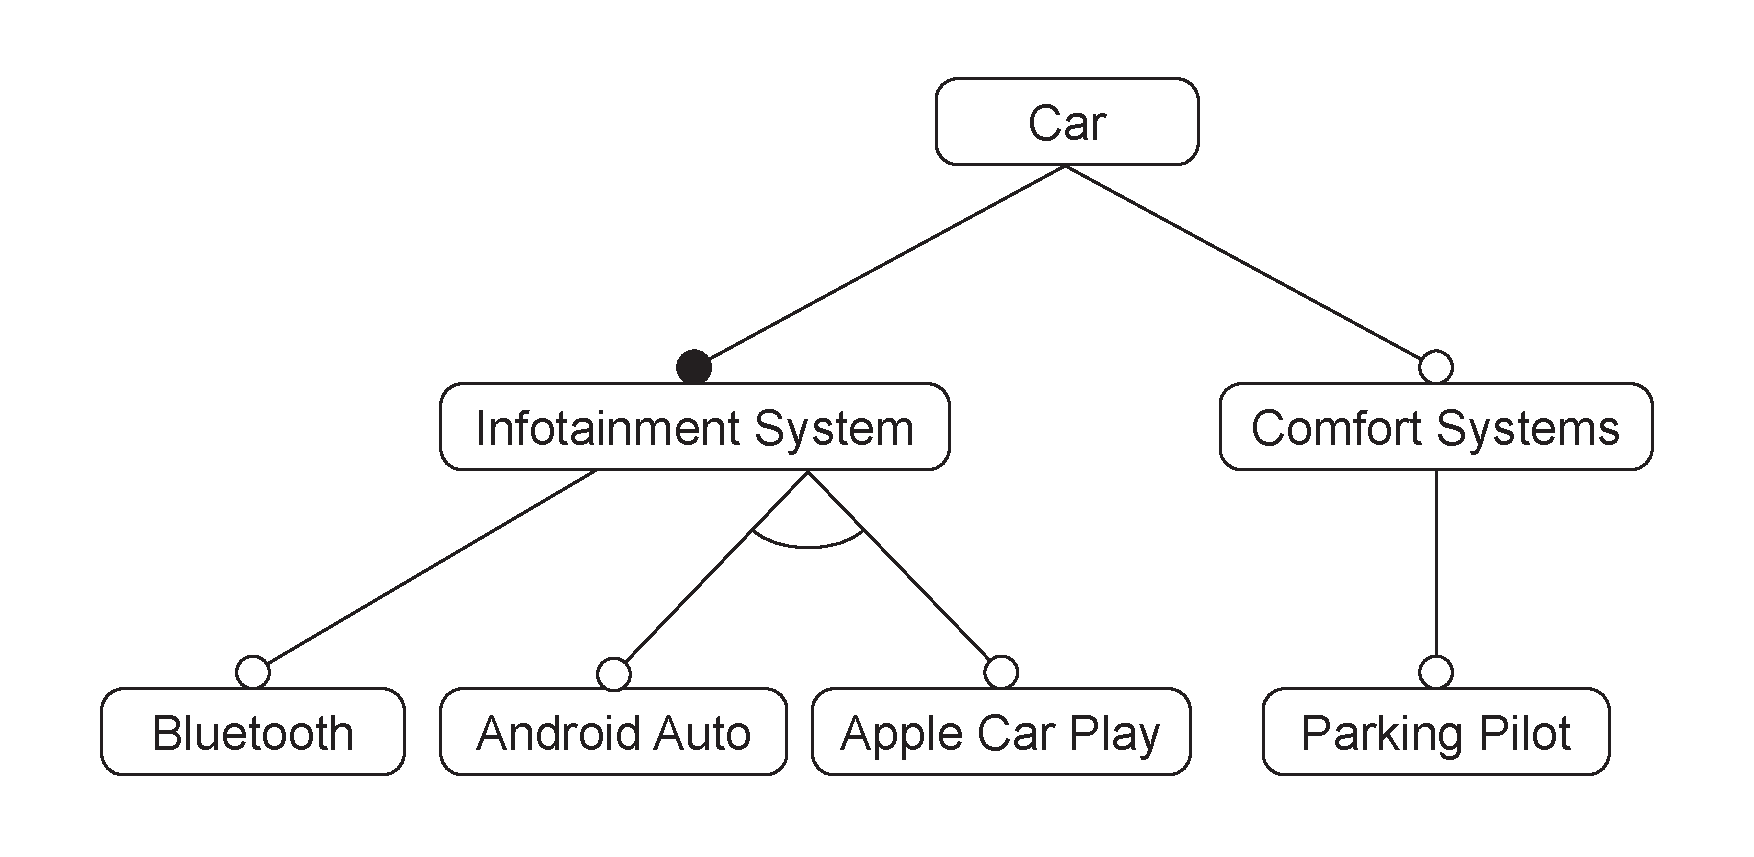
\includegraphics[width=0.8\linewidth]{illustrations/example.pdf}
	\caption{Example feature model}%
	\label{fig:example1}
\end{figure}

A visual representation of a feature model can be seen in Figure~\vref{fig:example1}. The small dot above \texttt{Infotainment System} indicates that the feature is mandatory, where as the white dot above \texttt{Comfort Systems} represents an optional feature. Each feature (except the root) is in a group. The \texttt{Infotainment System} feature is in a singleton group below \texttt{Car}. The features \texttt{Android Auto} and \texttt{Apple Car Play} are in a \texttt{XOR} group, indicated by the arch between the features. This represents that each valid variant has to choose between one of the two (but not both).

\section{Evolution planning}%
\label{sec:evolution_planning}

Feature models let engineers capture all variants of the current software product line, but sometimes it can be beneficial to model future or past versions as well. Planning for the long term evolution of the product line can be important in managing the complexity that comes with large software systems. Developing these kinds of systems typically involves many engineers, managers or other stakeholders, and managing when certain changes, additions or deprecations are implemented can be complex and confusing without suitable tools. Changing the SPL potentially influences many configurations, which might conflict with the stakeholders requirements.

SPL evolution is a major challenge in SPL engineering as many stakeholders are involved, many requirements exist, and changing the SPL potentially influences many configurations. Thus, it is paramount to thoroughly plan SPL evolution in advance, e.g., to perform analyses and to have enough time for implementing new or adapted features.

\textit{Evolution plans} lets us model a sequence of feature models, which represents the current and all planned future versions of the feature model. Each feature model represents the product line in a point in time, which could have varying validity, from a week from now to a year. Since the next feature model is derived from the previous one, we can represent the evolution plan as an initial feature model, as well as a sequence of \textit{points}, where each point is a set of operations to perform on the previous feature model to achieve the current one. The operations vary from changing, adding or deleting features or groups from the feature model.

\begin{figure}[htpb]
	\centering
	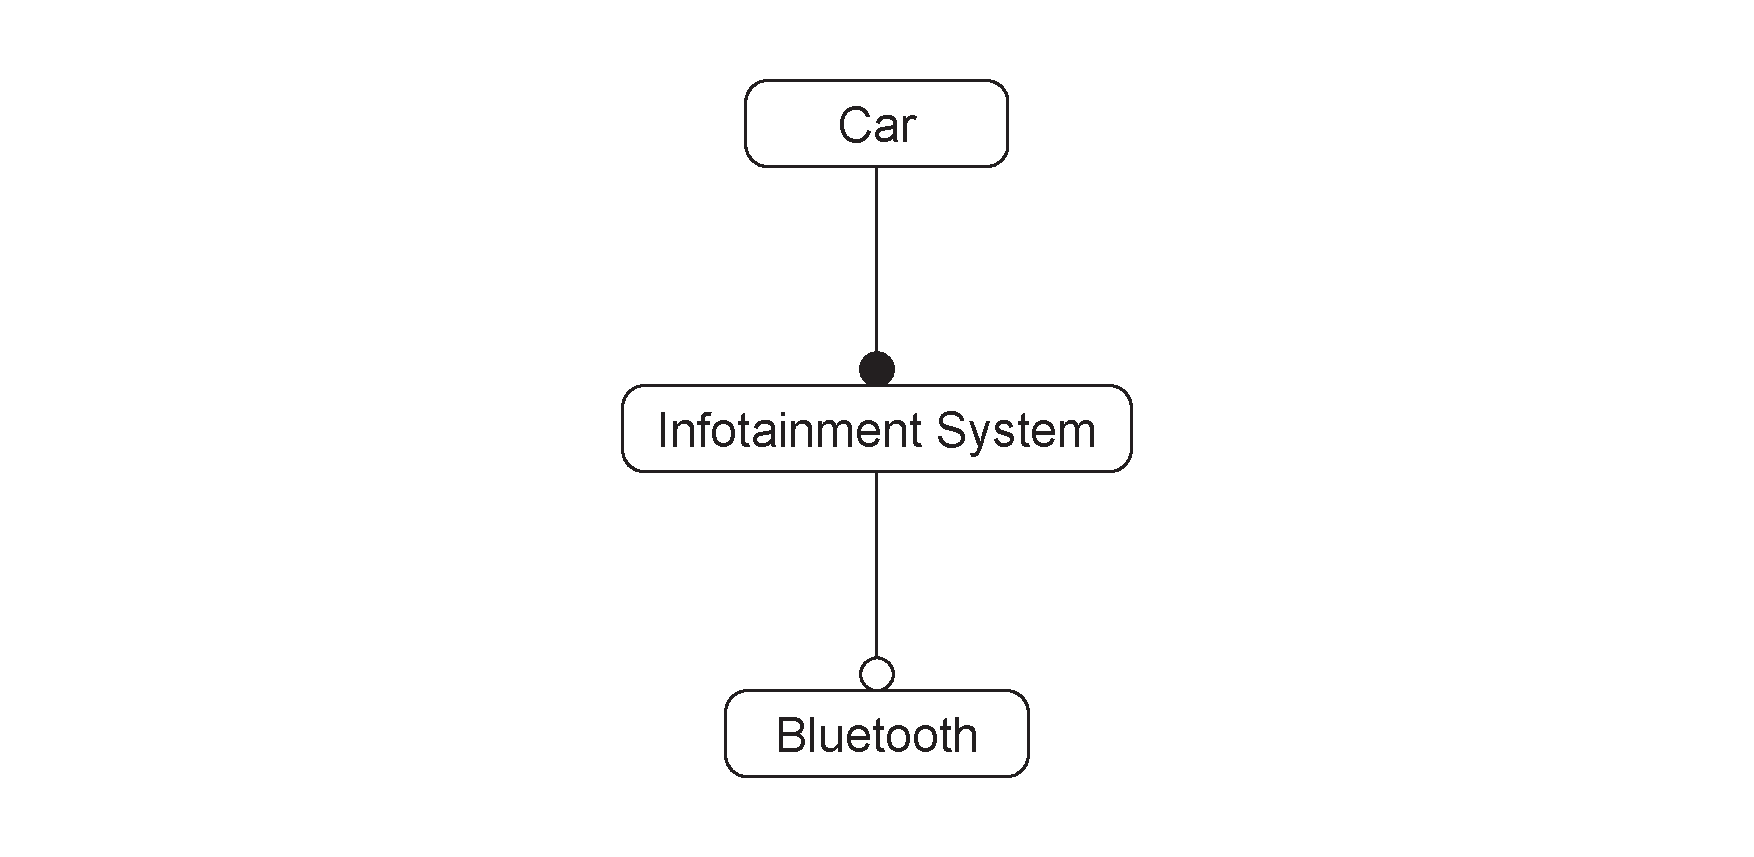
\includegraphics[width=0.8\linewidth]{illustrations/initial.pdf}
	\begin{tabular}{l}
		\textbf{At time 1:}                                           \\ \hline
		add an XOR group to Infotainment System.                      \\
		add feature Android Auto to the Infotainment System XOR group \\
		add feature Car Play to the Infotainment System XOR group     \\
		\\
		\textbf{At time 2:}                                           \\ \hline
		add feature Comfort Systems to the Car AND group              \\
		add an AND group to Comfort Systems                           \\
		add feature Parking Pilot to the Comfort Systems AND group
	\end{tabular}
	\caption{An example evolution plan}%
	\label{fig:exampleplan}
\end{figure}

An example of an evolution plan can be seen in Figure~\vref{fig:exampleplan}. The initial feature model contains three features, and two time points are added. At time 1, a group and two features are added, and at time 2, another group and two features are added. The evolution plan can derive three feature models, the initial, and the two at time 1 and 2. Performing all the operations results in a feature model that is equal to the one in Figure~\vref{fig:example1}

\section{Version Control Systems}%
\label{sec:version_control_systems}

\textit{Software configuration mechanisms} is the discipline of managing the evolution of large and complex software systems \cite{cite:software_configuration_management}. \textit{Version control mechanisms} are used to deal with the evolution of software products. These mechanisms include ways to deal with having multiple, parallel versions of the software simultaneously. Techniques like \textit{software merging} are used to keep consistency and unify different versions by automatically or semi-automatically deriving merged versions of the different parallel versions.

Mens~\cite{cite:tom_mens_software_merging_survey} categorizes and describes different aspect of version control systems and software merging techniques. Two-way and three-way merging differentiates between how many versions of the artifact you are comparing. Different representations of the merge artifact can be categorized in textual, syntactic, semantic or structural merging. State-based merge techniques uses delta algorithms to compute differences between revisions while change-based techniques keeps track of the exact operations that were performed between the revisions.

\subsection{Two-way vs three-way merging}%
\label{sub:two_way_vs_three_way_merging}

When merging different versions of a piece of software, we differentiate between \textit{two-way} and \textit{three-way} merging. Two-way merging merges the two versions without taking a common ancestor into account. Three-way merging on the other hand, uses a common ancestor as a reference point, to know how the different versions were changed. The latter technique is more powerful and produces more accurate merges, because the merge will know extra information from the common ancestor.

To illustrate the difference, consider the following program: \texttt{print(a); print(b); print(a + b)}, and two different versions derived from the base program, (1) \texttt{print(a); print(b); print(a+b); print("new line")}, (2) \texttt{print(b); print(a + b)}. Since a three-way merger uses the base program as a reference point, it will notice that derived version 1 added one statement, while version two deleted one. The three-way merger will then merge successfully without conflict with the following result: \texttt{print(b); print(a + b); print("new line")}. However, a two-way merger does not use the base program the different versions were derived from, and can not deduce whether \texttt{print(a)} were added in version 1 or deleted in version 2, thus raising a conflict. The same ambiguity occurs with the added statement \texttt{print("new line")}.

\subsection{Textual merging}%
\label{sub:textual_merging}

Textual merging views the software artifacts as unstructured text files. There exist several granularities of what is considered one unit, but \textit{line-based merging} is probably the most common textual merge. Line-based merging techniques computes the difference between files by comparing equality over the lines. This has several implications, like adding a single space after a line is considered a deletion of the old line and addition of the new. This coarse granularity often leads to unnecessary and confusing conflicts. Changing the indentation or other formatting differences often lead to unnecessary conflicts.

To exemplify this, consider the two versions of a Python program, Listing~\vref{lst:code_diff_1} and Listing~\vref{lst:code_diff_2}. The second version simply wrapped the content of the function in an if-statement that checks for input sanity. Using a standard textual, line-based differencing tool like the Unix' \textit{diff}-tool \cite{cite:fast_algo_for_lcs}, we are able to calculate the difference between the two files by calculating the longest common subsequence. As seen in the result (Listing~\vref{lst:result_code_diff}), difference between the two are confusing and inaccurate. Conceptually, the difference is that the second version wrapped the block in a if-statement. Due to the coarse grained line-based differencing and the disregard of structure and semantics, the algorithm reports that the whole block is deleted, and the same block wrapped in an if is inserted.

\begin{listing}
	\begin{minted}[]{python}
def some_function(n):
  sum = 0
  for i in range(0, n):
    sum += i
  print(sum)
some_function(5)

  \end{minted}
	\caption{Code diff 1}
	\label{lst:code_diff_1}
\end{listing}

\begin{listing}
	\begin{minted}[]{python}
def some_function(n):
  if isinstance(n, int):
    sum = 0
    for i in range(0, n):
      sum += i
    print(sum)
some_function(5)
  \end{minted}
	\caption{Code diff 2}
	\label{lst:code_diff_2}
\end{listing}

\begin{listing}
	\begin{minted}{text}
<   sum = 0
<   for i in range(0, n):
<     sum += i
<   print(sum)
---
>   if isinstance(n, int):
>     sum = 0
>     for i in range(0, n):
>       sum += i
>     print(sum)
  \end{minted}
	\caption{Resulting code diff}
	\label{lst:result_code_diff}
\end{listing}

As discussed, text-based merge techniques often provide inferior results, however, they have several advantages in terms of efficiency and generality. The algorithm is general enough to work well for different programming languages, documentation, markup files, configuration files, etc. Some measurements performed on three-way, textual, line-based merge techniques in industrial case studies showed that about 90 percent of the changed files could be merged automatically \cite{cite:large_scale_case_study}. Other tools can complement the merge algorithm in avoiding or resolving conflicts. Formatters can make sure things like indentation and whitespace are uniformly handled, to avoid unnecessary conflicts. Compilers can help in resolving conflicts arising from things like renaming, where one version renames a variables, while another version introduces new lines referencing the old variable.

\subsection{Syntactic Merging}%
\label{sub:syntactic_merging}

\textit{Syntactic merging}~\cite{cite:syntactic_software_merging} differs from textual merging in that it considers the syntax of the artifact it is merging. This makes it more powerful, because depending on the syntactic structure of the artifact, the merger can ignore certain aspects, like whitespace or code comments. Syntactic merge techniques can represent the software artifacts in a better data structure than just flat text files, like a tree or a graph. In example, representing the Python program from Listing~\vref{lst:code_diff_1} and Listing~\vref{lst:code_diff_2} as a parse tree or abstract syntax tree, we can avoid merge conflicts.

The granularity of the merger is still relevant, because we sometimes want to report a conflict even though the versions can be automatically merged. Consider the following example. $n < x$ is changed to $n \leq x$ in one version, and to $n < x + 1$ in another. Too fine grained granularity may cause this to be merged conflict free as $n \leq x + 1$. The merge can be done automatically and conflict free, but here we want to report a warning or conflict, because the merge might lead to logical errors.

\subsection{Semantic Merging}%
\label{sub:semantic_merging}

While syntactic merging is more powerful than its textual counterpart, there are still conflicts that go unnoticed. The syntactical mergers can detect conflicts explicitly encoded in the tree structure of the software artifact, however, there often exist implicit, cross-tree constraints in the software. An example of such a constraint is references to a variable. The variable references in the code are often semantically tied to the definition of the variable, where the name and scope implicitly notes the cross tree reference to the definition.

Consider the following simple program: \texttt{var i; i = 10;}. If one version changes the name of the variable: \texttt{var num; num = 10;}, and another version adds a statement referencing the variable: \texttt{var i; i = 10; print(i)}. Syntactic or textual mergers would not notice the conflict arising due to the implicit cross-tree constraints regarding the variable references, and merge the versions conflict-free with the following, syntactically valid result: \texttt{var num; num = 10; print(i)}.

Semantic mergers takes these kinds of conflicts into consideration while merging. Using \textit{Graph-based}  or \textit{context-sensitive} merge techniques, we can model such cross tree constraints, by linking definitions and invocations with edges in the graph. However, in some cases, such \textit{static semantic} merge techniques are not sufficient. Some changes cannot generally be detected statically, and may need to rely on the runtime semantics.

\section{Haskell and Algebraic Data Types}%
\label{sec:haskell_and_algebraic_data_types}

\todo{write about type synonyms, data types including records and sum types. show polymorphic data types. maybe something about deriving, maybe lens generation? etc. something about maybe? expressive and strict type system}

\section{Problem Definition}%
\label{sec:problem_definition}

\chapter{Formal Semantics of Feature Model Evolution Plans}%
\label{cha:formal_semantics_of_feature_model_evolution_plans}

As stated in \textbf{RQ2} in section~\vref{sec:research_questions}, we want design the merger in a way that guarantees a sound merge result. In order to do so, we need to have a clear, formal definition of the software artifact at hand, namely feature model evolution plans.

The formal structure and semantics of evolution plans are defined in a paper published in the Software Product Line Conference (SPLC)\footnote{https://splc.net/}, which I was fortunate enough to contribute to \cite{cite:consistency_preserving_evolution_planning}. The paper defines the evolution plan as an initial feature model, together with an ordered list of planning sections containing all edit operations that are scheduled for the same time point. The edit operations include addition and deletion of features and groups, as well as modifications to their fields, such as names or types. For every operation, we defined what makes an operation valid or invalid according to the formal definitions of feature models. 

In the work in this thesis, I will build upon, alter and extend the definitions and semantics of evolution plans defined in the other work I have contributed to. The semantics of editing operations were defined to create a soundness checker for evolution plans, which is used as a tool aiding replanning of evolution plans. However, since the focus of this thesis is to harmonize different alterations to evolution plan, we will need to adapt the evolution plan representation to fit this task.

\section{Issues with using a list-based approach}%
\label{sec:issues_with_using_a_list_based_approach}

In our work on creating a soundness checker for evolution plans, we used a representation where the ordering of the operations for a single point in time mattered. This list-based approach of grouping operations had several advantages regarding the formal definition of sound evolution plans as well as implementation-specific concerns. In defining what was considered a well-defined operation, we considered only the current feature model and the operation at hand. What order the user applied the operations did not really matter, as long as applying each operation resulted in a sound evolution plan.

However, when we design an approach to merging two evolution plans, the exact way each feature model in the evolution plan was derived is besides the point. The only thing the user sees are a list of feature models associated with time points. Exactly how the evolution plan was manipulated, and in what order each editing operation took place is not relevant for the user, so it should also not be relevant for the merge algorithm. As described in \textbf{RQ3} in section~\ref{sec:research_questions}, we want to produce merge results that are predictable and transparent. Having a list-based approach might make it hard to differentiate equal plans. Since there often is more than one way of going from one feature model to another, seemingly equal evolution plans might be represented differently.

Since part of the goal is to produce a sound result, we cannot simply rearrange the ordering of operations without complications. Some operations might be dependent on other operations, and rearranging the operations might result in an unsound plan. 

To counter these issues, one might naïvely find an standardized ordering of operations so one could sort the operations, or simply just store them as a set of operations instead of a list. However, as we will see, the order of the operations still matter, and changing the ordering can have varying effects. We observe three different ordering related scenarios for operations; non-dependent operations, dependent operations, and shadowed operations. By swapping the operations in a plan, you might achieve one of these scenarios. In the following sections, We investigate the scenarios in the following sections, which is also illustrated in Figure~\ref{fig:operation_swap_effect}.

\subsection*{Non-dependent Operations}%
\label{sub:non_dependent_operations}

In some cases, swapping the order of the operations in a time point has no effect on the resulting feature model. To exemplify this, take a simple feature model with two features and a group, organized in the following way: $\texttt{Root} \rightarrow \texttt{G1} \rightarrow \texttt{F1}$. In the following time point, there is scheduled a removal of feature \texttt{F1} as well as a name change for the root feature \texttt{Root} to \texttt{F0}. Applying both operations should yield the following feature model: $\texttt{F0} \rightarrow \texttt{G1}$. Since there is no structural or semantic relation between the operations, the order of when they are applied makes no difference. With the current list-based representation of a plan for a single time point, there are two ways of representing the changes. You could either schedule the removal of the \texttt{F1} feature first, or the name change of the root feature first. 

\begin{figure}[htpb]
  \centering
  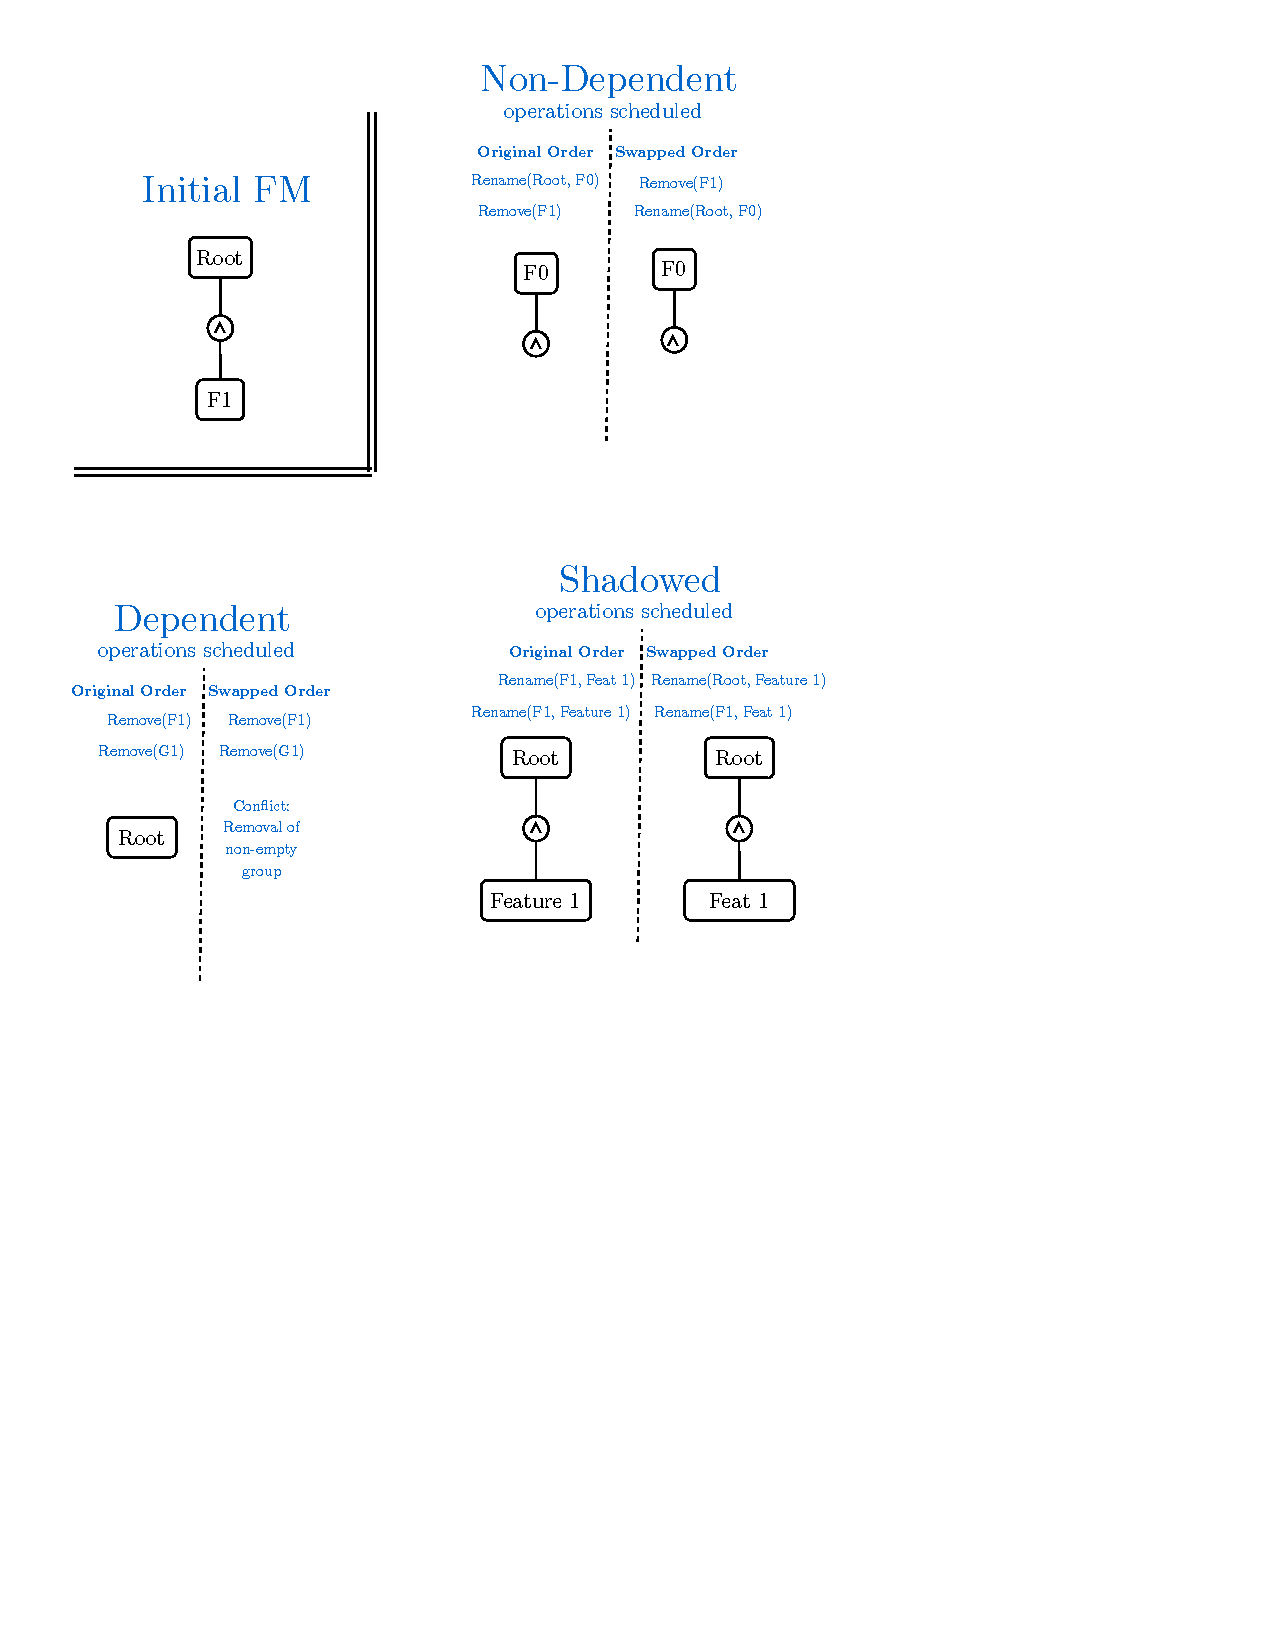
\includegraphics[width=0.8\linewidth]{operation_swap_effect.pdf}
  \caption{The various effects of swapping the ordering of operations}%
  \label{fig:operation_swap_effect}
\end{figure}

\subsection*{Dependent Operations}%
\label{sub:dependent_operations}

To showcase the problem, we start with the same feature model used previously, with two features and a group: $\texttt{Root} \rightarrow \texttt{G1} \rightarrow \texttt{F1}$. In the next planned time point, the changes to the feature model include the removal of both group \texttt{G1} and feature \texttt{F1}. However, there is only one legal ordering, namely removing the feature first, then removing the group. Applying the operation in this order yields a sound feature model; $\texttt{Root}$. Trying to remove the group first will as we defined sound evolution plans yield an inconsistency, because we are trying to remove a non-empty group. 

\subsection*{Operation Shadowing}%
\label{sub:operation_shadowing}

Another issue with the list-based approach is \textit{operation shadowing}, which is the phenomenon where an operation is rendered useless because of another operation later in the list. This issue would also have to be considered, because rearranging the operation could lead to unwanted results. In addition to rearrangement resulting in unsound plans, moving a shadowed operation might result in a different, yet sound evolution plan.

We exemplify operation shadowing, we consider the same initial feature model as before: $\texttt{Root} \rightarrow \texttt{G1} \rightarrow \texttt{F1}$. The list of operations for the next point in time include first changing the name of \texttt{F1} to \texttt{Feat 1}, then later to \texttt{Feature 1}. The operation shadowing occurs because of the second renaming makes the first renaming completely useless. The resulting feature model, $\texttt{Root} \rightarrow \texttt{G1} \rightarrow \texttt{Feature 1}$, are identical to the one we would have if we excluded the shadowed operation. However, if we were to swap the ordering of the rename operations, the resulting feature model would still be sound, but differ from the original ordering: $\texttt{Root} \rightarrow \texttt{G1} \rightarrow \texttt{Feat 1}$.

\section{Constructing a Normal Form for Evolution Plans}%
\label{sec:constructing_a_normal_form_for_evolution_plans}

In order to avoid the problems stated above, we construct a new representation for evolution plans. This representation is more aligned with what the user interacts with, so equal plans are also represented equally. In this representation, called \texttt{TreeUserEvolutionPlan}, the evolution plan is represented as a list of feature models together with a time point. Instead of storing the operations necessary to go from the previous time point to the next, each feature model is explicitly encoded. Each feature model is represented as a mutually recursive tree structure of features and groups. This representation is the normal form of evolution plans, and the closest representation to what the user actually interacts with.

The exact representation of \texttt{TreeUserEvolutionPlan} are defined formally in the Haskell code. Haskell's powerful type system with records and algebraic data types allows for a pretty precise formalization. When presented here in the thesis, the types are somewhat simplified, leaving out unnecessary noise, such as automatically derived instances for JSON serialization, equality checking, etc.

\subsection{Feature Model Definition - Tree Representation}%
\label{sub:feature_model_definition_tree_representation}

First, we will look at the tree representation for feature models, formalized as \texttt{TreeFeatureModel}.

\begin{minted}{haskell}
data TreeFeatureModel = TreeFeatureModel
  { rootFeature :: TreeFeature
  }

data TreeFeature = TreeFeature
  { id :: FeatureId
  , featureType :: FeatureType
  , name :: String
  , groups :: Set TreeGroup
  }

data TreeGroup = TreeGroup
  { id :: GroupId
  , groupType :: GroupType
  , features :: Set TreeFeature
  }

data FeatureType
  = Optional
  | Mandatory

data GroupType
  = And
  | Or
  | Alternative

type FeatureId = String

type GroupId = String
\end{minted}

There is a few important things to note in this representation. Each feature and groups id is unique across the entire feature model, which we will leverage when merging. Each feature and group can have an arbitrary number of children. The children is organized in a \texttt{Set}, not a \texttt{List}, noting that the ordering is irrelevant. In order for the feature model to be sound, some combination of parent group type and child feature types are prohibited. If a group is of type \texttt{Alternative} or \texttt{Or}, every child feature has to be of type \texttt{Optional}.

\subsection{Evolution Plan Definition - User Level Representation}%
\label{sub:evolution_plan_definition_user_level_representation}

\subsubsection*{Polymorphic User Level Evolution Plan}%
\label{ssub:polymorphic_user_level_evolution_plan}

Now that we have a suitable definition feature models, we define evolution plans. In this representation, we want the evolution plans to mirror what the user interacts with, so we define the evolution plan as a list of feature models. In later stages of the merge algorithm, we will reuse this \textit{user level} definition of evolution plans, only with a different definition of feature models. This allows us to leverage Haskell's polymorphic type system, which spares us from defining it twice.

\begin{minted}{haskell}
data UserEvolutionPlan featureModel = UserEvolutionPlan
  { timePoints :: [TimePoint featureModel]
  }

type Time = Int

data TimePoint featureModel = TimePoint
  { time :: Time
  , featureModel :: featureModel
  }
\end{minted}

\subsubsection*{Instantiated User Level Evolution Plan (Tree Feature Model)}%
\label{ssub:instantiated_user_level_evolution_plan_tree_feature_model_}



Now that a generalized representation for evolution plans are defined, using a representation with a list of feature models, we can instantiate the polymorphic evolution plan to create our normal form, \texttt{TreeUserEvolutionPlan}. This is relatively straight forward, the only thing we have to do is replace the \texttt{featureModel} argument with our concrete feature model, namely \texttt{TreeFeatureModel}.

\begin{minted}{haskell}
type TreeUserEvolutionPlan = UserEvolutionPlan TreeFeatureModel
\end{minted}

\subsection{Example Representation}%
\label{sub:example_representation}

Now that we have defined the normal form for evolution plans formally, we will give a concrete example and how it is represented in this formalization. The example we will showcase is a small example containing three time points. The initial feature model at time 0 is simply just the root feature. The next time point at time 1 adds a new group and two features belonging to this group. The last time point removes one of the features and alters the name of the root and type of the group. A visualization of this simple evolution plan can be seen in Figure~\vref{fig:simpleep_treeuser}. Below is the Haskell code necessary for encoding this example.

\begin{minted}{haskell}
simpleExample :: TreeUserEvolutionPlan
simpleExample =
  UserEvolutionPlan
    [ TimePoint 0 fm0
    , TimePoint 1 fm1
    , TimePoint 2 fm2
    ]
  where
    fm0 =
      TreeFeatureModel
        ( TreeFeature
            "rootFeature"
            Mandatory
            "Feature 1"
            Set.empty
        )
    fm1 =
      TreeFeatureModel
        ( TreeFeature
            "rootFeature"
            Mandatory
            "Feature 1"
            ( Set.fromList
                [ TreeGroup
                    "group"
                    And
                    ( Set.fromList
                        [ TreeFeature
                            "feature2"
                            Optional
                            "Feature 2"
                            Set.empty
                        , TreeFeature
                            "feature3"
                            Mandatory
                            "Feature 3"
                            Set.empty
                        ]
                    )
                ]
            )
        )
    fm2 =
      TreeFeatureModel
        ( TreeFeature
            "rootFeature"
            Mandatory
            "Root Feature"
            ( Set.fromList
                [ TreeGroup
                    "group"
                    Or
                    ( Set.fromList
                        [ TreeFeature
                            "feature2"
                            Optional
                            "Feature 2"
                            Set.empty
                        ]
                    )
                ]
            )
        )
\end{minted}

\begin{figure}[htpb]
  \centering
  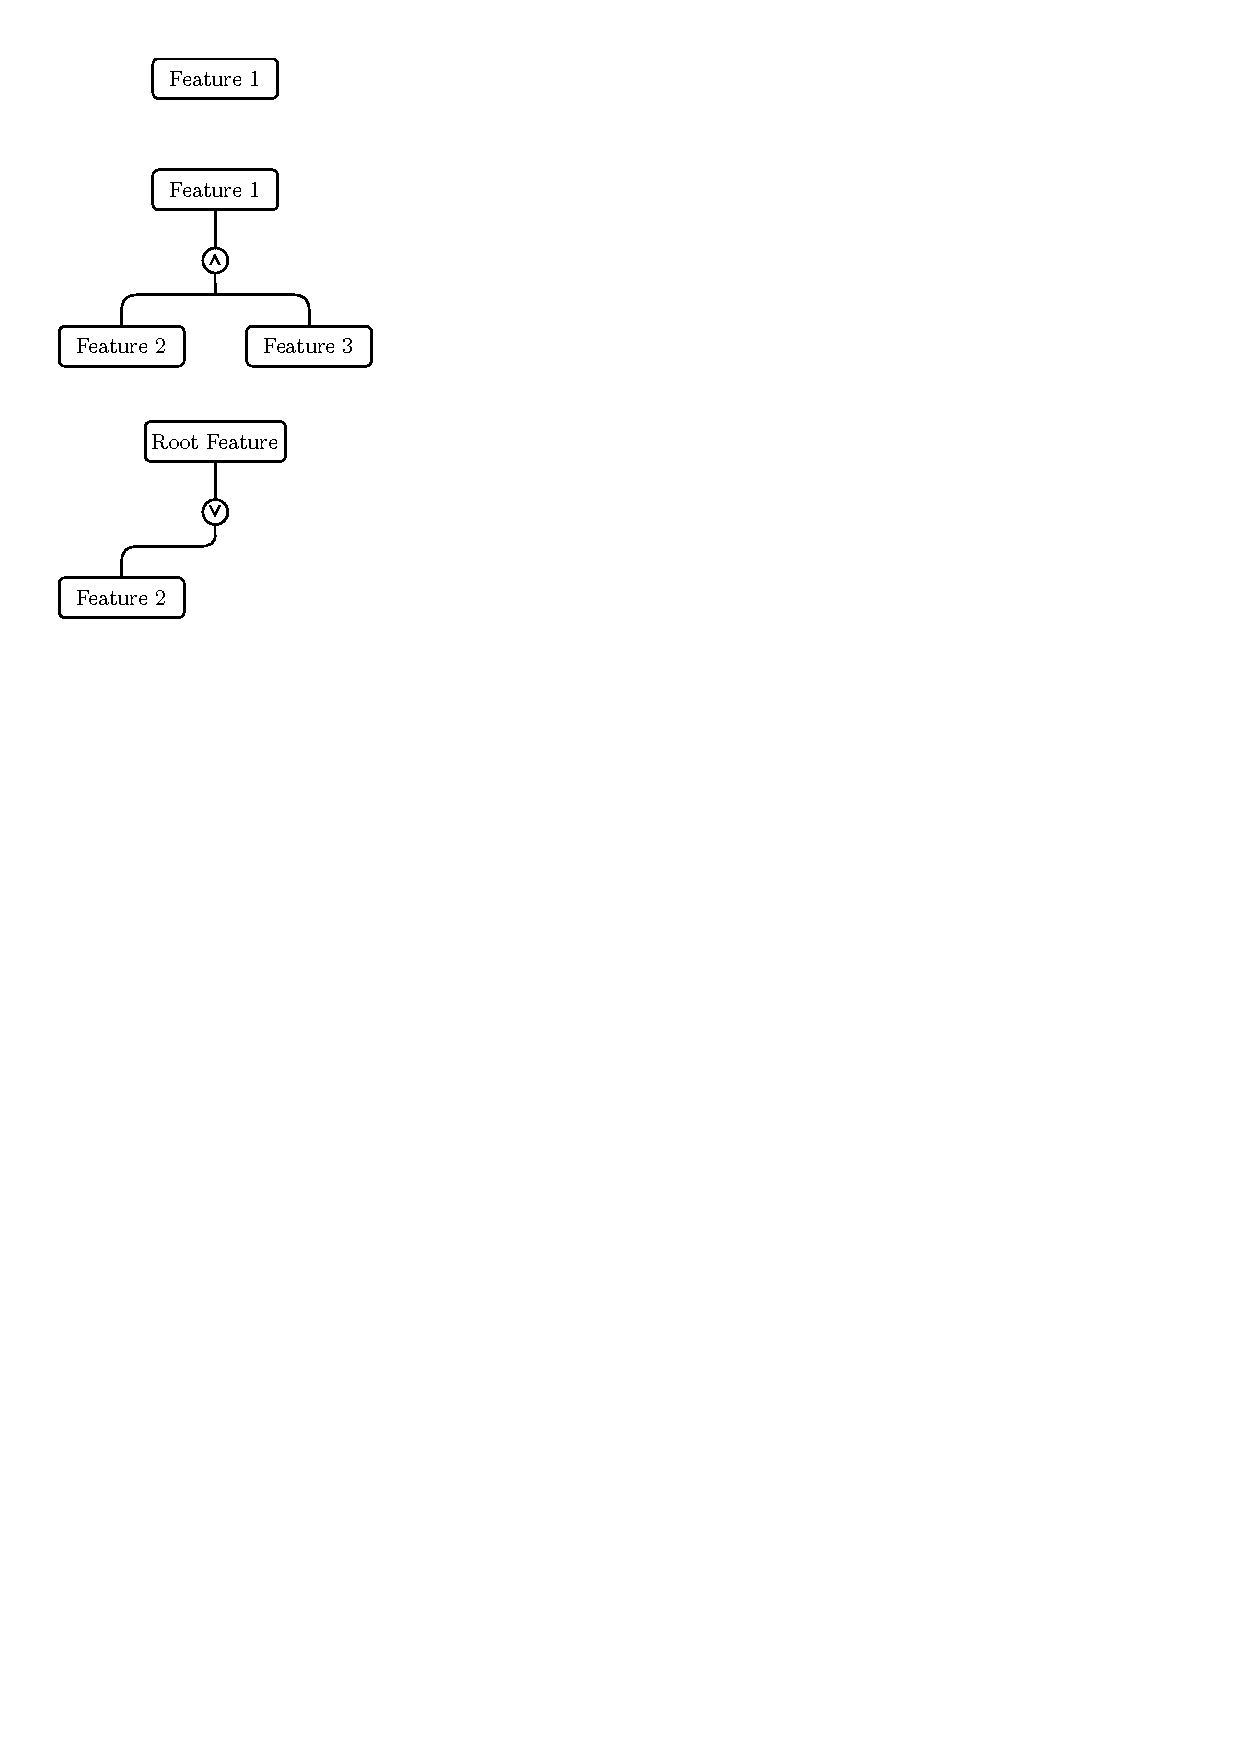
\includegraphics[]{simpleep_treeuser.pdf}
  \caption{A Simple Evolution Plan Example}%
  \label{fig:simpleep_treeuser}
\end{figure}

\section{A Suitable Representation of Evolution}%
\label{sec:a_suitable_representation_of_evolution}

The evolution plan formalization defined above, \texttt{TreeUserEvolutionPlan}, works well for capturing the essence of evolution plans. It represents evolution plans in terms of what the user actually deals with. However, in order to do an effective merge of two evolution plans, we need to represent the evolution plan a bit differently.

Refactoring the evolution plan doesn't just involve modifying the last time point, but replanning the other time points earlier in the plan. When users are replanning such time points, the additions, deletions and modifications has an effect not just on the time point at hand, but all subsequent time points. When a user adds a new feature in the middle of the plan, the feature would appear on the specified time points as well as all the time points beyond. When calculating the changes made, we don't want to look at this like a feature was added in all the time points, but rather just the specified time. In order to capture the essence of the changes made to each evolution plan, we would need to find a representation capturing the actual changes more explicitly.

In order to to capture the explicit modifications between each time point in the evolution plan, we would need to figure out an approach to calculating the difference between two subsequent feature models. However, with our current tree-based feature model, \texttt{TreeFeatureModel}, this can be a bit cumbersome, requiring us to traverse the two trees simultaneously. In some cases this is not very straight forward, i.e. handling \texttt{Move}-operations that relocates entire subtrees.

\subsection{Feature Model Definition - Flat Representation}%
\label{sub:feature_model_definition_flat_representation}

We define a new representation for feature models, \texttt{FlatFeatureModel}, in order to have a structure better suited for detecting and applying changes to the tree-structure. This is achievable due to our features and groups having unique ids. This allows for a simple mapping-structure, where we each feature and group can be looked up by its id. The edges and relations in the tree are modeled as node-id references instead of a recursive structure. Every node only stores its parent relation, not its child relations as well. This makes moving entire subtrees straight forward, requiring changing only the parent-field of the node to move.

\begin{minted}{haskell}
data FlatFeatureModel = FlatFeatureModel
  { rootId :: FeatureId
  , features :: Map FeatureId FlatFeature
  , groups :: Map GroupId FlatGroup
  }

data FlatFeature = FlatFeature
  { parentGroupId :: Maybe GroupId
  , featureType :: FeatureType
  , name :: String
  }

data FlatGroup = FlatGroup
  { parentFeatureId :: FeatureId
  , groupType :: GroupType
  }
\end{minted}

The definition of \texttt{FeatureType}, \texttt{FeatureId}, \texttt{GroupType} and \texttt{GroupId} is still the same as defined in Section~\vref{sub:feature_model_definition_tree_representation}.

\todo{The new definition of feature models also has advantages we will exploit when defining a new.......... something about temporarily damaging..}

\todo{something about it allowing for modifications that temporarily  damage the structure. one could add a child before adding the parent, if you know for certain that the resulting plan is correct}

\subsection{Evolution Plan Definition - Modification Level Representation}%
\label{sub:evolution_plan_definition_modification_level_representation}

% As discussed in Section~\ref{sec:issues_with_using_a_list_based_approach}, the list-based operation approach is problematic in order to achieve a desired merge result.

% An important part in merging the efforts of two collaborators is figuring out exactly what changes each collaborators did to the common base evolution plan. With our current representation of evolution plans, \texttt{TreeUserEvolutionPlan}, detecting changes in the tree can be quite difficult.




\todo{kan snakke om operasjonene, hva de betyr på høynivå. referere til artikkel for detaljer.}
\todo{arbeid er basert på sunn plan.}

\chapter{Three Way Merge Algorithm}%
\label{cha:three_way_merge_algorithm}

\section{Algorithm Overview}%
\label{sec:algorithm_overview}

\subsection{Three-Way Merging of Evolution Plans}%
\label{sub:three_way_merging_of_evolution_plans}

The three-way merge algorithm for feature model evolution plans will take two different versions of an evolution plan, \textit{version 1} and \textit{version 2}, and attempt to merge the evolution plans into a single plan. In order to do so, a third evolution plan has to be provided, which is the common evolution plan they were derived from. The common evolution plan, called \textit{base}, will implicitly provide information about what things were added, removed and changed in each of the derived evolution plans.

\subsection{Soundness Assumption}%
\label{sub:soundness_assumption}

The three-way merge algorithm will assume that the three evolution plans provided are sound. By assuming the soundness of the plans, the algorithm can leverage this to create a better merge result. But more importantly, the assumption is based around the fact that there is no point in merging an evolution plan you know violates soundness in some way.

\subsection{Algorithm Phases}%
\label{sub:algorithm_phases}

In order to merge the different versions of the evolution plan, the algorithm is separated into several distinct phases. The different steps and phases of the algorithm can be seen in Figure~\ref{fig:merge_outline}.

\begin{figure}[htbp]
  \centering
  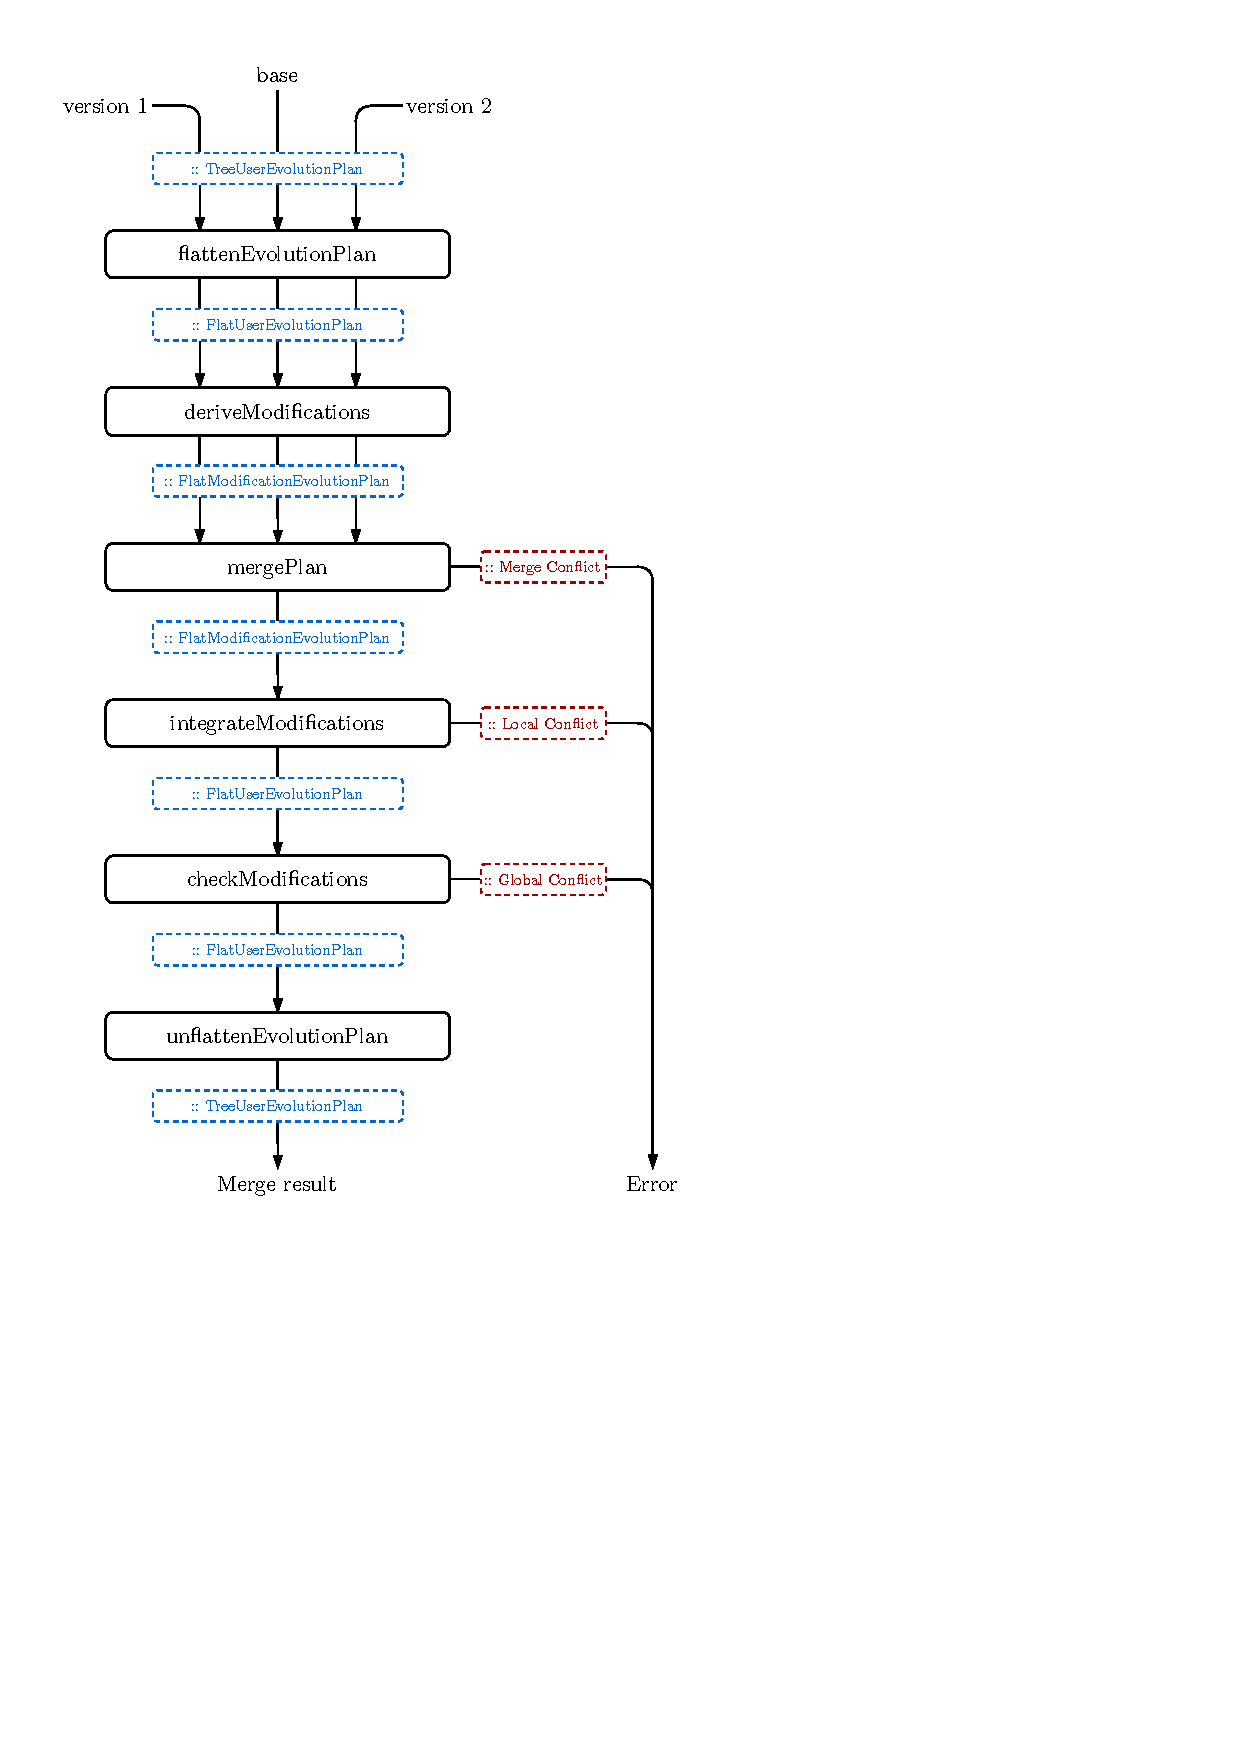
\includegraphics[width=0.8\linewidth]{merge_outline}
  \caption{Outline of the three-way merge algorithm}%
  \label{fig:merge_outline}
\end{figure}

The first phase is transforming the three different evolution plans into representations that is more suitable for merging. This includes converting both the way feature models are represented as well as the way the entire evolution plan is represented. This phase includes the \texttt{flattenEvolutionPlan} and \texttt{deriveModifications}, which is described in further detail in \vref{sec:converting_to_a_suitable_representation}

After changing the way evolution plans are represented, the second phase of the algorithm will calculate the differences between the \textit{base} evolution plan and both derived evolution plans, \textit{version 1}, and \textit{version 2}. This will let us know what were added, changed and removed in each of the derived evolution plans. This phase is part of the \texttt{mergePlan} function, which is described in further detail in \vref{sec:detecting_the_changes_between_versions}

The information from the previous phase will be used to create a single merged evolution plan. This evolution plan is simply just the \textit{base} evolution plan integrated with all the changes from \textit{version 1} and \textit{version 2}. This phase is part of the \texttt{mergePlan} function, which is described in further detail in \vref{sec:merging_intended_changes}

Now that a single merged evolution plan is provided, the last step is to ensure that the plan is following the structural and semantic requirements of an evolution plan. Merging all changes from both versions might yield various inconsistencies. This includes structural conflicts such as orphan features, entire subtrees forming cycles, removing non-empty features, etc. The last phase includes converting back to the original representation, as well as ensuring soundness while doing so. This phase is part of the \texttt{integrateModifications}, \texttt{checkModifications} and \texttt{unflattenEvolutionPlan} functions, which is explained further in \vref{sec:ensuring_structural_and_semantic_soundness_of_merge_result}

\subsection{Conflicts}%
\label{sub:conflicts}

During the different phases of the merge algorithm, different kind of conflicts or errors could occur. Depending on what part of the algorithm a conflict occurred, the conflicts might be either a \textit{merge}, \textit{local} or \textit{global} conflict. At what phase each conflict could occur can also be seen in Figure~\vref{fig:merge_outline}, but a short description of the different conflicts are described below. 

\textit{Merge Conflicts} occur because of conflicting operations on a single feature or group. This could happen if one version tries to remove a feature, while the other tries to change the type of a feature. This could also happen if there originally existed a modification in the \textit{base} version, and one of the derived versions try to change the modification, while the other tries to remove the modification.

\textit{Local Conflicts} occur when a modification is not possible to be applied because of the existence or non-existence of a feature or group. For example, if we try to add a feature with an id that already exist, or try to change the type of a group that does not exist.

\textit{Global Conflicts} is the last kind of error that could occur. When all the modifications has been integrated into the evolution plan, each feature model is checked for certain structural or semantical errors. At this point, each change \textit{local} to a feature or group is valid, so we check for potential errors that occur because of dependencies between the features and groups, \textit{global} to the entire feature model. The structural errors is typically modifications that lead to anomalies in the tree structure. These violations of the structure could happen if you add features to parents that don't exist, remove groups that has children, or move features in such a way that cycles are formed. Other violations to the semantics are also checked. This could for example be violations of well-formedness, that could happen if we change the type of a feature to something incompatible with its group.

\section{Converting To a Suitable Representation}%
\label{sec:converting_to_a_suitable_representation}

\subsection{Representing Feature Models}%
\label{sub:representing_feature_models}

\subsection{Representing Evolution Plans}%
\label{sub:representing_evolution_plans}

\section{Detecting the Changes Between Versions}%
\label{sec:detecting_the_changes_between_versions}

\section{Merging Intended Changes}%
\label{sec:merging_intended_changes}

\section{Ensuring structural and semantic soundness of the merge result}%
\label{sec:ensuring_structural_and_semantic_soundness_of_merge_result}

\chapter{Example Merge – Vending Machine}%
\label{cha:example_merge_vending_machine}

write about the vending machine example. Write about how the entire example is done. from cli parsing, converting to right representation, merging, checking, converting back, writing to file. Then how the frontend visualization tool parses the result and displays the tree as an interactive  thing.

sound vs unsound examples

\chapter{Conclusion and Future Work}%
\label{cha:conclusion_and_future_work}

konklusjon bør si hvordan det jeg har gjort addresserer forskningsspørsmålene
forskningsspørsmålene kan være større en bidraget
how to ensure sound plan and merge of sound plans

future work kan være flere ting å se på for å belyse forskningsspm

\backmatter{}

\printbibliography

\end{document}
